% SoC architecture block diagram (Fig. 1).
% Build: pdflatex fig1_soc_block.src.tex && mv fig1_soc_block.src.pdf fig1_soc_block.pdf
\documentclass[border=2pt]{standalone}
\usepackage{mathptmx}
\usepackage{tikz}
\usetikzlibrary{arrows.meta,positioning,calc,shapes.geometric}

\definecolor{navy}{HTML}{1F3A5F}
\definecolor{tlgred}{HTML}{A83232}
\definecolor{redfill}{HTML}{F4DADA}

\begin{document}
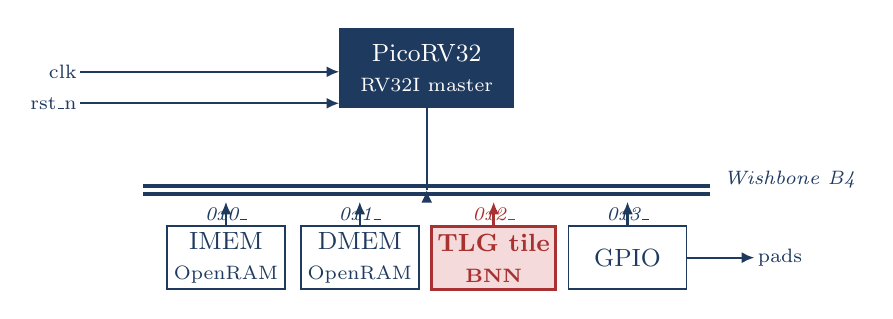
\begin{tikzpicture}[
    font=\rmfamily,
    >={Latex[length=1.6mm,width=1.4mm]},
    line width=0.6pt,
    primary/.style  = {draw=navy,   fill=navy,    text=white, line width=0.6pt,
                       minimum height=8mm, minimum width=15mm, align=center,
                       inner sep=2pt, font=\rmfamily\small},
    secondary/.style= {draw=navy,   fill=white,   text=navy,  line width=0.6pt,
                       minimum height=8mm, minimum width=15mm, align=center,
                       inner sep=2pt, font=\rmfamily\small},
    tlg/.style      = {draw=tlgred, fill=redfill, text=tlgred, line width=1.0pt,
                       minimum height=8mm, minimum width=15mm, align=center,
                       inner sep=2pt, font=\rmfamily\small\bfseries},
    bus/.style      = {draw=navy, line width=1.4pt},
    sig/.style      = {draw=navy, line width=0.8pt, ->},
    redsig/.style   = {draw=tlgred, line width=1.2pt, ->},
    addr/.style     = {font=\rmfamily\scriptsize\itshape, text=navy, inner sep=1pt},
    pin/.style      = {font=\rmfamily\scriptsize, text=navy, inner sep=1pt},
  ]

  % --- Master ----------------------------------------------------------
  \node[primary, minimum width=22mm, minimum height=10mm] (cpu)
    at (0,0) {PicoRV32\\\scriptsize RV32I master};

  % --- Wishbone bus (horizontal) ---------------------------------------
  \coordinate (busL) at (-3.6,-1.6);
  \coordinate (busR) at ( 3.6,-1.6);
  \draw[bus] (busL) -- (busR);
  \draw[bus] ($(busL)+(0,0.10)$) -- ($(busR)+(0,0.10)$);
  \node[font=\rmfamily\scriptsize\itshape, text=navy, anchor=west]
    at ($(busR)+(0.05,0.18)$) {Wishbone B4};

  % CPU drop to bus
  \draw[sig] (cpu.south) -- ++(0,-0.6) |- ($(busL)!0.5!(busR)+(0,0.05)$);

  % --- Slaves ----------------------------------------------------------
  \node[secondary, anchor=north] (imem) at (-2.55,-2.0) {IMEM\\\scriptsize OpenRAM};
  \node[secondary, anchor=north] (dmem) at (-0.85,-2.0) {DMEM\\\scriptsize OpenRAM};
  \node[tlg,       anchor=north] (tile) at ( 0.85,-2.0) {TLG tile\\\scriptsize BNN};
  \node[secondary, anchor=north] (gpio) at ( 2.55,-2.0) {GPIO};

  % Address decode labels above each slave
  \node[addr, anchor=south] at ($(imem.north)+(0,0.02)$) {0x0\_};
  \node[addr, anchor=south] at ($(dmem.north)+(0,0.02)$) {0x1\_};
  \node[addr, anchor=south, text=tlgred]
                                   at ($(tile.north)+(0,0.02)$) {0x2\_};
  \node[addr, anchor=south] at ($(gpio.north)+(0,0.02)$) {0x3\_};

  % Bus drops to each slave
  \foreach \n in {imem,dmem,gpio}{
    \draw[sig] (\n.north) -- ++(0,0.30);
  }
  \draw[redsig] (tile.north) -- ++(0,0.30);

  % --- External I/O ----------------------------------------------------
  \draw[sig] (-4.4,-0.05) -- (cpu.west |- 0,-0.05);
  \draw[sig] (-4.4,-0.45) -- (cpu.west |- 0,-0.45);
  \node[pin, anchor=east] at (-4.4,-0.05) {clk};
  \node[pin, anchor=east] at (-4.4,-0.45) {rst\_n};

  \draw[sig] (gpio.east) -- ++(0.85,0);
  \node[pin, anchor=west] at ($(gpio.east)+(0.85,0)$) {pads};

\end{tikzpicture}
\end{document}
